\documentclass[twoside]{book}

% Packages required by doxygen
\usepackage{fixltx2e}
\usepackage{calc}
\usepackage{doxygen}
\usepackage[export]{adjustbox} % also loads graphicx
\usepackage{graphicx}
\usepackage[utf8]{inputenc}
\usepackage{makeidx}
\usepackage{multicol}
\usepackage{multirow}
\PassOptionsToPackage{warn}{textcomp}
\usepackage{textcomp}
\usepackage[nointegrals]{wasysym}
\usepackage[table]{xcolor}

% Font selection
\usepackage[T1]{fontenc}
\usepackage[scaled=.90]{helvet}
\usepackage{courier}
\usepackage{amssymb}
\usepackage{sectsty}
\renewcommand{\familydefault}{\sfdefault}
\allsectionsfont{%
  \fontseries{bc}\selectfont%
  \color{darkgray}%
}
\renewcommand{\DoxyLabelFont}{%
  \fontseries{bc}\selectfont%
  \color{darkgray}%
}
\newcommand{\+}{\discretionary{\mbox{\scriptsize$\hookleftarrow$}}{}{}}

% Page & text layout
\usepackage{geometry}
\geometry{%
  a4paper,%
  top=2.5cm,%
  bottom=2.5cm,%
  left=2.5cm,%
  right=2.5cm%
}
\tolerance=750
\hfuzz=15pt
\hbadness=750
\setlength{\emergencystretch}{15pt}
\setlength{\parindent}{0cm}
\setlength{\parskip}{3ex plus 2ex minus 2ex}
\makeatletter
\renewcommand{\paragraph}{%
  \@startsection{paragraph}{4}{0ex}{-1.0ex}{1.0ex}{%
    \normalfont\normalsize\bfseries\SS@parafont%
  }%
}
\renewcommand{\subparagraph}{%
  \@startsection{subparagraph}{5}{0ex}{-1.0ex}{1.0ex}{%
    \normalfont\normalsize\bfseries\SS@subparafont%
  }%
}
\makeatother

% Headers & footers
\usepackage{fancyhdr}
\pagestyle{fancyplain}
\fancyhead[LE]{\fancyplain{}{\bfseries\thepage}}
\fancyhead[CE]{\fancyplain{}{}}
\fancyhead[RE]{\fancyplain{}{\bfseries\leftmark}}
\fancyhead[LO]{\fancyplain{}{\bfseries\rightmark}}
\fancyhead[CO]{\fancyplain{}{}}
\fancyhead[RO]{\fancyplain{}{\bfseries\thepage}}
\fancyfoot[LE]{\fancyplain{}{}}
\fancyfoot[CE]{\fancyplain{}{}}
\fancyfoot[RE]{\fancyplain{}{\bfseries\scriptsize Generated by Doxygen }}
\fancyfoot[LO]{\fancyplain{}{\bfseries\scriptsize Generated by Doxygen }}
\fancyfoot[CO]{\fancyplain{}{}}
\fancyfoot[RO]{\fancyplain{}{}}
\renewcommand{\footrulewidth}{0.4pt}
\renewcommand{\chaptermark}[1]{%
  \markboth{#1}{}%
}
\renewcommand{\sectionmark}[1]{%
  \markright{\thesection\ #1}%
}

% Indices & bibliography
\usepackage{natbib}
\usepackage[titles]{tocloft}
\setcounter{tocdepth}{3}
\setcounter{secnumdepth}{5}
\makeindex

% Hyperlinks (required, but should be loaded last)
\usepackage{ifpdf}
\ifpdf
  \usepackage[pdftex,pagebackref=true]{hyperref}
\else
  \usepackage[ps2pdf,pagebackref=true]{hyperref}
\fi
\hypersetup{%
  colorlinks=true,%
  linkcolor=blue,%
  citecolor=blue,%
  unicode%
}

% Custom commands
\newcommand{\clearemptydoublepage}{%
  \newpage{\pagestyle{empty}\cleardoublepage}%
}

\usepackage{caption}
\captionsetup{labelsep=space,justification=centering,font={bf},singlelinecheck=off,skip=4pt,position=top}

%===== C O N T E N T S =====

\begin{document}

% Titlepage & ToC
\hypersetup{pageanchor=false,
             bookmarksnumbered=true,
             pdfencoding=unicode
            }
\pagenumbering{roman}
\begin{titlepage}
\vspace*{7cm}
\begin{center}%
{\Large run-\/on-\/courseB }\\
\vspace*{1cm}
{\large Generated by Doxygen 1.8.11}\\
\end{center}
\end{titlepage}
\clearemptydoublepage
\tableofcontents
\clearemptydoublepage
\pagenumbering{arabic}
\hypersetup{pageanchor=true}

%--- Begin generated contents ---
\chapter{Class Index}
\section{Class List}
Here are the classes, structs, unions and interfaces with brief descriptions\+:\begin{DoxyCompactList}
\item\contentsline{section}{\hyperlink{classSerial}{Serial} }{\pageref{classSerial}}{}
\end{DoxyCompactList}

\chapter{File Index}
\section{File List}
Here is a list of all documented files with brief descriptions\+:\begin{DoxyCompactList}
\item\contentsline{section}{include/{\bfseries serial.\+hpp} }{\pageref{serial_8hpp}}{}
\item\contentsline{section}{src/\hyperlink{line__tracer_8cpp}{line\+\_\+tracer.\+cpp} \\*Line trace programm }{\pageref{line__tracer_8cpp}}{}
\item\contentsline{section}{src/\hyperlink{serial_8cpp}{serial.\+cpp} \\*\hyperlink{classSerial}{Serial} communication module for Linux to send commands to mbot }{\pageref{serial_8cpp}}{}
\end{DoxyCompactList}

\chapter{Class Documentation}
\hypertarget{classSerial}{}\section{Serial Class Reference}
\label{classSerial}\index{Serial@{Serial}}
\subsection*{Public Member Functions}
\begin{DoxyCompactItemize}
\item 
{\bfseries Serial} (std\+::string port\+\_\+name)\hypertarget{classSerial_a9c4cb307f3b68213d98bc71636c1ea5c}{}\label{classSerial_a9c4cb307f3b68213d98bc71636c1ea5c}

\item 
void {\bfseries write\+\_\+command} (std\+::string command)\hypertarget{classSerial_acbf8f4424b3f1215bec7b6c2877511ac}{}\label{classSerial_acbf8f4424b3f1215bec7b6c2877511ac}

\end{DoxyCompactItemize}


The documentation for this class was generated from the following files\+:\begin{DoxyCompactItemize}
\item 
include/serial.\+hpp\item 
src/\hyperlink{serial_8cpp}{serial.\+cpp}\end{DoxyCompactItemize}

\chapter{File Documentation}
\hypertarget{line__tracer_8cpp}{}\section{src/line\+\_\+tracer.cpp File Reference}
\label{line__tracer_8cpp}\index{src/line\+\_\+tracer.\+cpp@{src/line\+\_\+tracer.\+cpp}}


Line trace programm.  


{\ttfamily \#include \char`\"{}serial.\+hpp\char`\"{}}\\*
{\ttfamily \#include \char`\"{}opencv2/highgui/highgui.\+hpp\char`\"{}}\\*
{\ttfamily \#include \char`\"{}opencv2/imgproc/imgproc.\+hpp\char`\"{}}\\*
{\ttfamily \#include $<$iostream$>$}\\*
{\ttfamily \#include $<$sstream$>$}\\*
{\ttfamily \#include $<$chrono$>$}\\*
{\ttfamily \#include $<$sys/time.\+h$>$}\\*
{\ttfamily \#include $<$sys/ioctl.\+h$>$}\\*
{\ttfamily \#include $<$fcntl.\+h$>$}\\*
{\ttfamily \#include $<$unistd.\+h$>$}\\*
Include dependency graph for line\+\_\+tracer.\+cpp\+:
\nopagebreak
\begin{figure}[H]
\begin{center}
\leavevmode
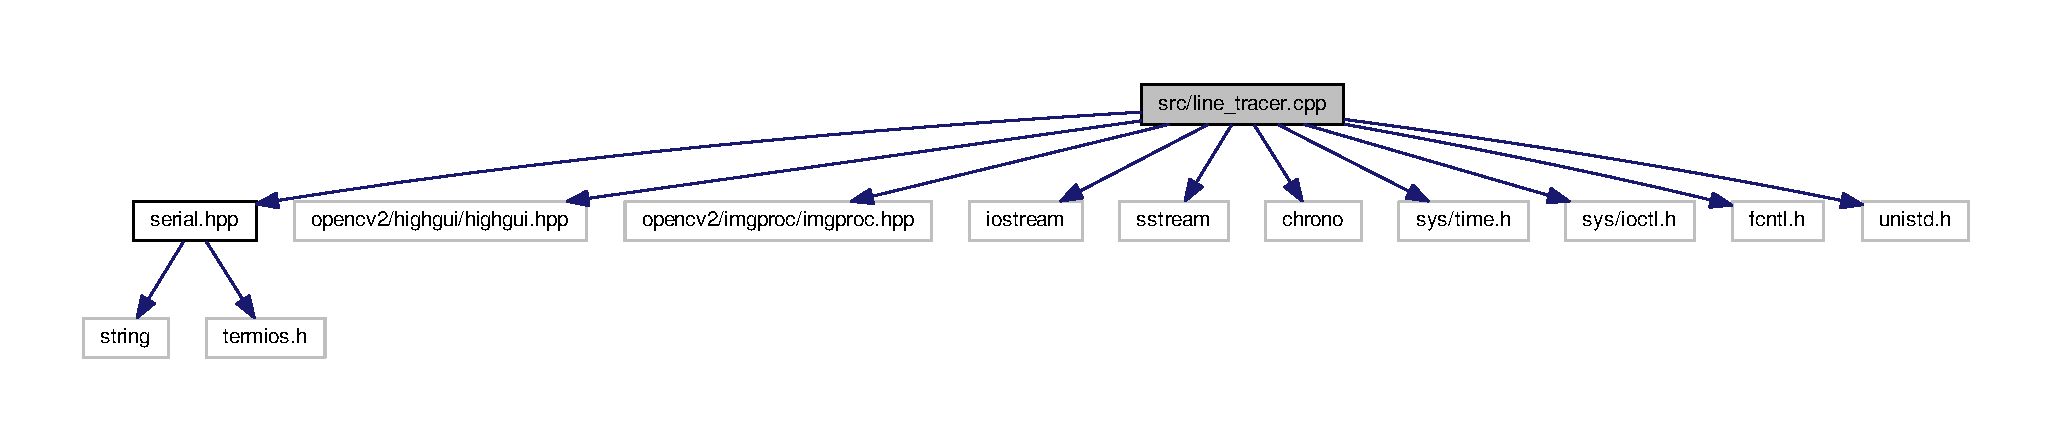
\includegraphics[width=350pt]{line__tracer_8cpp__incl}
\end{center}
\end{figure}
\subsection*{Functions}
\begin{DoxyCompactItemize}
\item 
const string \hyperlink{line__tracer_8cpp_aa10d13c46fc27ae1de1e146c6500b590}{S\+E\+R\+I\+A\+L\+\_\+\+P\+O\+RT} (\char`\"{}/dev/tty\+U\+S\+B0\char`\"{})\hypertarget{line__tracer_8cpp_aa10d13c46fc27ae1de1e146c6500b590}{}\label{line__tracer_8cpp_aa10d13c46fc27ae1de1e146c6500b590}

\begin{DoxyCompactList}\small\item\em Arduino uno device port. \end{DoxyCompactList}\item 
void {\bfseries binalize\+\_\+image} (Mat \&src\+\_\+img, Mat \&dst\+\_\+img)\hypertarget{line__tracer_8cpp_a5843c4ed067d6d2701481c46f702d165}{}\label{line__tracer_8cpp_a5843c4ed067d6d2701481c46f702d165}

\item 
void {\bfseries count\+\_\+white\+\_\+pixels} (Mat \&image, int $\ast$ave\+\_\+of\+\_\+pix\+\_\+val, int $\ast$edge\+\_\+pix\+\_\+idx)\hypertarget{line__tracer_8cpp_aee271cdb4d6c5ad8104d2a679eee1af7}{}\label{line__tracer_8cpp_aee271cdb4d6c5ad8104d2a679eee1af7}

\item 
void {\bfseries update\+\_\+state} (\hyperlink{classSerial}{Serial} ser, int ave\+\_\+of\+\_\+pix\+\_\+val, int edge\+\_\+pix\+\_\+idx)\hypertarget{line__tracer_8cpp_ab13fa819908194cfcde2a1f1b59b569f}{}\label{line__tracer_8cpp_ab13fa819908194cfcde2a1f1b59b569f}

\item 
int {\bfseries main} (int argc, char $\ast$$\ast$argv)\hypertarget{line__tracer_8cpp_a3c04138a5bfe5d72780bb7e82a18e627}{}\label{line__tracer_8cpp_a3c04138a5bfe5d72780bb7e82a18e627}

\end{DoxyCompactItemize}
\subsection*{Variables}
\begin{DoxyCompactItemize}
\item 
const int \hyperlink{line__tracer_8cpp_a447efb7d562d7dd631b6a985ff88b5e0}{S\+P\+E\+ED} = 100\hypertarget{line__tracer_8cpp_a447efb7d562d7dd631b6a985ff88b5e0}{}\label{line__tracer_8cpp_a447efb7d562d7dd631b6a985ff88b5e0}

\begin{DoxyCompactList}\small\item\em motor base speed \end{DoxyCompactList}\item 
const int \hyperlink{line__tracer_8cpp_a56c8b1c930d21b18ab01f027401d05a4}{T\+A\+R\+G\+ET} = 30\hypertarget{line__tracer_8cpp_a56c8b1c930d21b18ab01f027401d05a4}{}\label{line__tracer_8cpp_a56c8b1c930d21b18ab01f027401d05a4}

\begin{DoxyCompactList}\small\item\em target x px \end{DoxyCompactList}\item 
const int \hyperlink{line__tracer_8cpp_a22889a0e83ef2e401d35d49c4bc1f9af}{KP} = 1.\+7\hypertarget{line__tracer_8cpp_a22889a0e83ef2e401d35d49c4bc1f9af}{}\label{line__tracer_8cpp_a22889a0e83ef2e401d35d49c4bc1f9af}

\begin{DoxyCompactList}\small\item\em coefficient for propotional control \end{DoxyCompactList}\item 
const double {\bfseries S\+T\+O\+P\+\_\+\+T\+I\+ME} = 3.\+0\hypertarget{line__tracer_8cpp_add7d6ba7ac0358626cdef9cefbea6bf5}{}\label{line__tracer_8cpp_add7d6ba7ac0358626cdef9cefbea6bf5}

\item 
const speed\+\_\+t \hyperlink{line__tracer_8cpp_a0302c316ec1bb7fd0ac27b926ca113fc}{B\+A\+U\+D\+R\+A\+TE} = B9600\hypertarget{line__tracer_8cpp_a0302c316ec1bb7fd0ac27b926ca113fc}{}\label{line__tracer_8cpp_a0302c316ec1bb7fd0ac27b926ca113fc}

\begin{DoxyCompactList}\small\item\em baudrate to communicate with Arduino uno \end{DoxyCompactList}\item 
const int {\bfseries W\+H\+I\+TE} = 255\hypertarget{line__tracer_8cpp_a6fdc54ca55874b2959f7d77967f78dc2}{}\label{line__tracer_8cpp_a6fdc54ca55874b2959f7d77967f78dc2}

\item 
const int {\bfseries B\+L\+A\+CK} = 0\hypertarget{line__tracer_8cpp_a5b27e565b0566bdf2097265d0987c156}{}\label{line__tracer_8cpp_a5b27e565b0566bdf2097265d0987c156}

\end{DoxyCompactItemize}


\subsection{Detailed Description}
Line trace programm. 

\begin{DoxyAuthor}{Author}
Kumikomi 
\end{DoxyAuthor}
\begin{DoxyDate}{Date}
05 Sep. 2018 
\end{DoxyDate}

\hypertarget{serial_8cpp}{}\section{src/serial.cpp File Reference}
\label{serial_8cpp}\index{src/serial.\+cpp@{src/serial.\+cpp}}


\hyperlink{classSerial}{Serial} communication module for Linux to send commands to mbot.  


{\ttfamily \#include \char`\"{}serial.\+hpp\char`\"{}}\\*
{\ttfamily \#include $<$iostream$>$}\\*
{\ttfamily \#include $<$stdio.\+h$>$}\\*
{\ttfamily \#include $<$sys/types.\+h$>$}\\*
{\ttfamily \#include $<$sys/stat.\+h$>$}\\*
{\ttfamily \#include $<$sys/ioctl.\+h$>$}\\*
{\ttfamily \#include $<$fcntl.\+h$>$}\\*
{\ttfamily \#include $<$termios.\+h$>$}\\*
{\ttfamily \#include $<$unistd.\+h$>$}\\*
Include dependency graph for serial.\+cpp\+:
\nopagebreak
\begin{figure}[H]
\begin{center}
\leavevmode
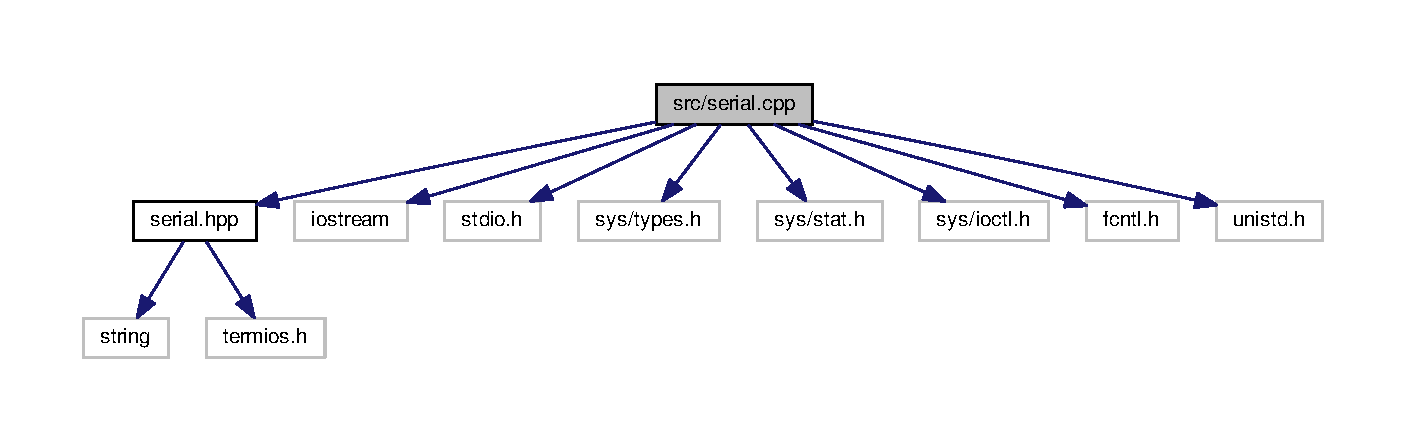
\includegraphics[width=350pt]{serial_8cpp__incl}
\end{center}
\end{figure}


\subsection{Detailed Description}
\hyperlink{classSerial}{Serial} communication module for Linux to send commands to mbot. 

\begin{DoxyAuthor}{Author}
Kenta Arai 
\end{DoxyAuthor}
\begin{DoxyDate}{Date}
05 Sep. 2018 
\end{DoxyDate}

%--- End generated contents ---

% Index
\backmatter
\newpage
\phantomsection
\clearemptydoublepage
\addcontentsline{toc}{chapter}{Index}
\printindex

\end{document}
